\documentclass{article}

\def\npart {II}
\def\nyear {2017}
\def\nterm {Lent}
\def\nlecturer{Prof. I. Grojnowski}
\def\ncourse{Algebraic Geometry}
\ifx \nauthor\undefined
  \def\nauthor{Bhavik Mehta}
\else
\fi

\author{Based on lectures by \nlecturer \\\small Notes taken by \nauthor}
\date{\nterm\ \nyear}
\title{Part \npart\ -- \ncourse}

\usepackage[utf8]{inputenc}
\usepackage{amsmath}
\usepackage{amsthm}
\usepackage{amssymb}
\usepackage{enumerate}
\usepackage{mathtools}
\usepackage{graphicx}
\usepackage[dvipsnames]{xcolor}
\usepackage{tikz}
\usepackage{wrapfig}
\usepackage{centernot}
\usepackage{float}
\usepackage{braket}
\usepackage[hypcap=true]{caption}
\usepackage{enumitem}
\usepackage[colorlinks=true, linkcolor=mblue]{hyperref}
\usepackage[nameinlink,noabbrev]{cleveref}
\usepackage{nameref}
\usepackage[margin=1.5in]{geometry}

% Theorems
\theoremstyle{definition}
\newtheorem*{aim}{Aim}
\newtheorem*{axiom}{Axiom}
\newtheorem*{claim}{Claim}
\newtheorem*{cor}{Corollary}
\newtheorem*{conjecture}{Conjecture}
\newtheorem*{defi}{Definition}
\newtheorem*{eg}{Example}
\newtheorem*{ex}{Exercise}
\newtheorem*{fact}{Fact}
\newtheorem*{law}{Law}
\newtheorem*{lemma}{Lemma}
\newtheorem*{notation}{Notation}
\newtheorem*{prop}{Proposition}
\newtheorem*{question}{Question}
\newtheorem*{rrule}{Rule}
\newtheorem*{thm}{Theorem}
\newtheorem*{assumption}{Assumption}

\newtheorem*{remark}{Remark}
\newtheorem*{warning}{Warning}
\newtheorem*{exercise}{Exercise}

% \newcommand{\nthmautorefname}{Theorem}

\newtheorem{nthm}{Theorem}[section]
\newtheorem{nlemma}[nthm]{Lemma}
\newtheorem{nprop}[nthm]{Proposition}
\newtheorem{ncor}[nthm]{Corollary}
\newtheorem{ndef}[nthm]{Definition}

% Special sets
\newcommand{\C}{\mathbb{C}}
\newcommand{\N}{\mathbb{N}}
\newcommand{\Q}{\mathbb{Q}}
\newcommand{\R}{\mathbb{R}}
\newcommand{\Z}{\mathbb{Z}}

\newcommand{\abs}[1]{\left\lvert #1\right\rvert}
\newcommand{\norm}[1]{\left\lVert #1\right\rVert}
\renewcommand{\vec}[1]{\boldsymbol{\mathbf{#1}}}

\let\Im\relax
\let\Re\relax

\DeclareMathOperator{\Im}{Im}
\DeclareMathOperator{\Re}{Re}
\DeclareMathOperator{\id}{id}

\definecolor{mblue}{rgb}{0., 0.05, 0.6}


% preamble
\usepackage{tikz}
\usepackage{stmaryrd}
\usepackage{tikz-cd}
\newcommand{\A}{\mathbb{A}}
\newcommand{\F}{\mathbb{F}}
\newcommand{\proj}{\mathbb{P}}
\DeclareMathOperator{\Mat}{Mat}
\DeclareMathOperator{\chara}{char}
\DeclareMathOperator{\Mor}{Mor}
\DeclareMathOperator{\Gal}{Gal}
%\setcounter{section}{-1}
% and here we go!

\begin{document}
\maketitle
\tableofcontents

Consider $E = \set{(x, y) \in \C^2 | y^2 = x^3 - x}$. Let's first draw this when $(x, y) \in \R^2$.
If $y \in \R$, $y^2 \geq 0$, so if $x \in \R$, $x^3 - x = x(x^2 - 1) \geq 0$ so $x \geq 1$ or $-1 \leq x \leq 0$.

% draw picture!

Now consider $(x, y) \in \C$. In general, this is tricky.
Here, define $p: E \to \C$ given by $(x, y) \mapsto x$ most of the time ($x \notin \{0, 1, -1\}$), $p^{-1}(x)$ is two points.
This doesn't help us visualise.

\begin{equation*}
    \Gamma = \set{(x, y) \in \C^2 | y \in \R, x \in [-1, 0] \cup [1, \infty)}
\end{equation*}
Claim: $E \setminus \Gamma$ is disconnected and has two pieces.
Proof: Exercise.

So, $E \setminus \Gamma$ is two copies of
% pic
glued together. To glue, turn one of the pieces over (this ruins the representation as a double cover, but is the right gluing).
Think of (the picture below) by adding a point at $\infty$, so it lives on the Riemann surface.

Take another copy, flip it over and glue back.
(this section is in the process of tidying)

\clearpage
% I
\section{Dictionary between algebra and geometry}
% 1.
\subsection{Basic notions}
\begin{defi}[Affine space]\label{def:affineSpace}
    \textbf{Affine $n$-space} is $\A^n = \A^n(k) \coloneqq k^n$ for $k$ a field.
\end{defi}
\begin{notation}\hypertarget{def:polys}
    Write $k[\A^n] = k[x_1, \dotsc, x_n]$ for the polynomials in $n$ variables.
\end{notation}
Any $f \in \hyperlink{def:polys}{k[\A^n]}$ defines a function $f: \A^n =k^n \to k$ given by $(\lambda_1, \dotsc, \lambda_n) \mapsto f(\lambda_1, \dotsc, \lambda_n)$ by evaluation.

Let $S \subseteq k[x_1, \dotsc, x_n]$ be any subset of polynomials.
\begin{defi}[Affine variety]\label{def:affineVariety}
    \begin{equation*}
        Z(S) = \set{\lambda = (\lambda_1, \dotsc, \lambda_n) \in k^n | f(\lambda_1, \dotsc, \lambda_n) = 0 \text{ for all } f \in S}
    \end{equation*}
    is called the \textbf{affine variety defined by} $S$, the simultaneous zeros of all functions in $S$.
    $Z(S)$ is called an affine subvariety of $\A^n$.
\end{defi}

\begin{eg}
    \leavevmode
    \begin{enumerate}[label=(\roman*)]
        \item $\hyperlink{def:affineSpace}{\A^n} = \hyperlink{def:affineVariety}{Z}(0)$.
        \item On $\A^1$, $Z(x) = \{0\}$, $Z(x-7) = \{7\}$.  If $f(x) = (x - \lambda_1)\dotsc (x-\lambda_n)$, $Z(f(x)) = \{\lambda_1, \dotsc, \lambda_n\}$.
            Affine subvarieties of $\A^1$ are: $\A^1$ and finite subsets of $\A^1$.
        \item in $\A^2$, $E=Z(y^2-x^3+x)$ we have sketched when $k=\C$ and $k=\R$ in the introduction.
            % diagrams of Z(x,y), Z(xy), Z(y) and Z(y(y-1),x(y-1))
    \end{enumerate}
\end{eg}

\begin{remark}
    If $f \in k[\A^n]$ then $Z(f)$ is called a \textbf{hypersurface}.
\end{remark}

Observe that if $J$ is the ideal generated by $S$
\begin{equation*}
    J = \Set{\sum a_i f_i | a_i \in k[x_1, \dotsc, x_n], f_i \in S}
\end{equation*}
then $Z(J) = Z(S)$.  Hence,
\begin{thm}
    If $Z(S)$ is an affine subvariety of $\A^n$, there is a finite set $f_1, \dotsc, f_r$ of polynomials with $Z(S) = Z(f_1, \dotsc, f_r)$.
\end{thm}

\begin{proof}
    $J = \langle f_1, \dotsc, f_r \rangle$ for some $f_1, \dotsc, f_r$ by Hilbert basis theorem.
\end{proof}

\begin{lemma}
    \leavevmode
    \begin{enumerate}[label=(\roman*)]
        \item if $I \subseteq J$, $Z(J) \subseteq Z(I)$
        \item $Z(0) = \A^n$, $Z(k[x_1, \dotsc, x_n]) = \emptyset$.
        \item $Z\left(\bigcup J_i\right) = Z(\sum J_i) = \bigcap Z(J_i)$ for any possibly infinite family of ideals
        \item $Z(I \cap J) = Z(I) \cup Z(J)$ if $I, J$ ideals
    \end{enumerate}
\end{lemma}
\begin{proof}
    (i), (ii), (iii) are clear.
    (iv): $\supseteq$ holds by (i). Conversely, if $x \notin Z(I)$ then $\exists f_1 \in I$ such that $f_1(x) \neq 0$.
    So if $x \notin Z(J)$ also, $\exists f_2 \in J$ with $f_2(x) \neq 0$ also.
    Hence $f_1 f_2(x) = f_1(x) f_2(x) \neq 0$, so $x \notin Z(f_1 f_2)$. But $f_1 f_2 \in I \cap J$, as $I, J$ ideals so $x \notin Z(I \cap J)$.
\end{proof}

Looking at these results, $Z(I)$ form closed subsets of a topology on $\A^n$, called the \hypertarget{def:zariski}{\textbf{`Zariski topology'}}.

If $Z \subset \A^n$ is any subset, let $I(Z) = \set{f \in k[\A^n] | f(p) = 0, \forall p \in Z}$.
Observe that $I(Z)$ is an ideal: if $g \in k[\A^n]$, $f(p) = 0$ then $(gf)(p) = 0$.
\begin{lemma}
    \leavevmode
    \begin{enumerate}[label=(\roman*)]
        \item $Z \subseteq Z' \implies I(Z') \subseteq I(Z)$
        \item for any $Y \subseteq \A^n$, $Y \subseteq Z(I(Y))$,
        \item if $V = Z(J)$ is a subvariety of $\A^n$, then $V = Z(I(V))$.
        \item if $J \lhd k[\A^n] = k[x_1, \dotsc, x_n]$ an ideal, then $J \subseteq I(Z(J))$.
    \end{enumerate}
\end{lemma}
\begin{proof}
    (i), (ii), (iv) are clear.
    For (iii), first show $\supseteq$. $I(V) = I(Z(J))\supseteq J$ by (iv) so $Z(I(V)) \subseteq Z(J)=V$ by (i). $\subseteq$ follows by (iv).
\end{proof}
Hence (ii) and (iii) show that $Z(I(Y))$ is the smallest affine subvariety of $\A^n$ containing $Y$, i.e. it is the closure of $Y$ in the Zariski topology.


Take $\Z \subseteq \C = \A^1$, $k = \C$.
If a polynomial in one variable vanishes at every integer, it is $0$, so $I(\Z) = 0$ and hence the closure of $\Z$ in the Zariski topology is $\C$.

Note if $k = \C$, $f \in \C[x_1, \dotsc, x_n]$, then $f$ is continuous in the usual topology, so
\begin{equation*}
    Z(J) = \bigcap_{f \in J} Z(f) = \bigcap_{f \in J} f^{-1}(\{0\})
\end{equation*}
is a closed set in the usual topology, i.e. Zariski closed $\implies$ closed in the usual topology.

So,
\begin{equation*}
\begin{tikzcd}
    \{\text{Zariski closed subvarieties of } \A^n\} \ar[r, bend right, hookrightarrow, "I"]& \{\text{ideals in } k[x_1, \dotsc, x_n]\} \ar[l, bend right, two heads, "Z"]
\end{tikzcd}
\end{equation*}
But this is not a bijection. For instance,
$Z(x) = Z(x^2) = Z(x^3) = \dotsc = \{0\} \subseteq \A^1$.
More generally,
$Z(\langle f_1^{a_1}, \dotsc, f_r^{a_r}\rangle) = Z(f_1, f_2, \dotsc, f_r)$.
but it turns out this kind of thing is the only problem.
This is called Hilbert's `Nullstellensatz'.
\begin{defi}
    An affine variety $Y$ is \textbf{reducible} if $\exists$ affine varieties $Y_1, Y_2$, $Y_i \neq Y$ with $Y = Y_1 \cup Y_2$, and irreducible otherwise, and disconnected if $Y_1 \cap Y_2 = \emptyset$.
\end{defi}
% picsss
So $Z(xy) = Z(x) \cup Z(y)$, reducible.
$Z(y(y-1), x(y-1)) = Z(x,y) \cup Z(y-1)$ reducible and disconnected.
\begin{prop}
    Any affine variety is a finite union of irreducible affine varieties.
\end{prop}
\begin{remark}
    This is very different from usual manifolds.
\end{remark}
\begin{proof}
    If not, $Y$ is not irreducible, so $Y = Y_1 \cup Y_1'$ and one of $Y_1, Y_1'$, (say $Y_1$) is not the finite union of irreducible affine varieties, so
    \begin{equation*}
        Y_1 = Y_2 \cup Y_2', \dotsc
    \end{equation*}
    and so we get an infinite chain of affine varities $Y \supsetneq Y_1 \supsetneq Y_2 \supsetneq \dotsb$.
    But each $Y_i = Z(I_i)$ for some ideal $I_l$. Let $W = \bigcap Y_l = Z(\sum I_i) = Z(I)$.
    $I = \sum I_i$ is an ideal. As the ideal $I$ is finitely generated $I = \langle f_1, \dotsc, f_r \rangle$ for some $f_i$.
    $f_i \in I_{a_i}$ for some $a_1, \dotsc, a_r$ so $I = I_{a_1} + \dotsb + I_{a_r}$, $W = Y_{i_1} \cap \dotsb \cap Y_{i_r}$ contradicting $Y_N \subsetneq Y_{a_1} \cap \dotsb \cap Y_{a_r}$ if $N > r$.
\end{proof}
\begin{ex}
    If $Y$ is a subvariety of $\A^\N$, $Y = Y_1 \cup \dotsb \cup Y_r$ with $Y_i$ irreducible, and $r$ minimal is unique up to reordering. Call the $Y_i$ the irreducible components of $Y$. % did you really mean \N?
\end{ex}
\begin{prop}
    $Y$ is irreducible $\iff I(Y)$ is a prime ideal in $k[\A^n] = k[x_1, \dotsc, x_n]$.
\end{prop}
\begin{eg}
    \leavevmode
    \begin{enumerate}[label=(\roman*)]
        \item $(x y)$ is not a prime ideal.
        \item Exercise: Let $R$ be a UFD, $f \in R$, $f \neq 0$, $f$ irreducible $\iff (f)$ a prime ideal.
        \item Exercise: $k[x_1, \dotsc, x_n]$ is a UFD.
            Hence $Z(y^2 - x^3 + x)$ is irreducible, $Z(y-x^2)$ is irreducible.
    \end{enumerate}
\end{eg}
\begin{proof}
    If $Y = Y_1 \cup Y_2$ is reducible, $\exists p \in Y_1 \setminus Y_2$ so $\exists f \in I(Y_2)$ such that $f(p) \neq 0$ and similarly, $\exists q \in Y_2 \setminus Y_1$ so $\exists g \in I(Y_1)$ such that $g(q) \neq 0$.
    Then $fg \in I(Y_1) \cap I(Y_2) = I(Y)$. But $f \notin I(Y)$, $g \notin I(Y)$ so not prime.
    \begin{center}
        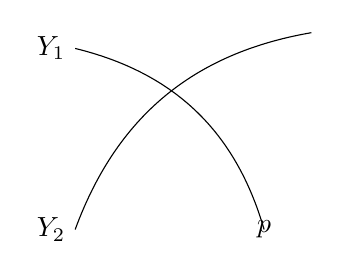
\begin{tikzpicture}
            \node [left] at (-1, 1.3) {$Y_1$};
            \node [left] at (-1, -1) {$Y_2$};
            \path (-1,1.3) edge [bend left=30] node[pos=1] {$p$} (1.4,-1) ;
            \draw (-1,-1) to[bend left=30] (2,1.5);
        \end{tikzpicture}
    \end{center}

    Conversely, if $I(Y)$ is not prime $\exists f_1 f_2 \in k[\A^n]$ such that $f_1, f_2 \notin I(Y)$ but $f_1 f_2 \in I(Y)$.
    Let $Y_i = Y \cap Z(f_i) = \set{p \in Y | f_i(p) = 0}$. $Y_1 \cup Y_2 = Y$, as $p \in Y \implies f_1 f_2 (p) = 0 \implies f_1(p) = 0$ or $f_2(p) = 0$.
    $Y_i \neq Y$ as $f_i \notin I(Y)$ (i.e. $\exists p_l \in Y$ such that $f_i(p_i) \neq 0$ so $p_i \notin Y_i$).
\end{proof}
\begin{lemma}
    $X$ irreducible affine subvariety of $\A^n$, $\mathcal{U} \subseteq X$ open and non-empty $\implies \overline{\mathcal{U}} = X$.
\end{lemma}
\begin{proof}
    Let $Y = X - \mathcal{U}$, closed. Then $\overline{\mathcal{U}} \cup Y = X$, and $\mathcal{U} \neq \emptyset \implies Y \neq X$. But $X$ is irreducible, so $\overline{\mathcal{U}} = X$.
\end{proof}

Application: Cayley-Hamilton Theorem
$A \in \Mat_n(k)$, an $n \times n$ matrix, with
\begin{equation*}
    \chara_A(x) = \det(x I - A) \in k[x]
\end{equation*}
the characteristic polynomial.
This gives a function $\chara_A: \Mat_n(k) \to \Mat_n(k)$ $B \mapsto \chara_A(B)$.
Cayley-Hamilton theorem says that $\forall A \in \Mat_n(k)$, $\chara_A(A) = 0$. Notice this is an equality of matrices, so it is $n^2$ equations.
\begin{proof}
    Let $X = \A^{n^2} = \Mat_n(k)$, affine space, hence irreducible algebraic variety.
    Consider $CH = \set{A \in \Mat_n(k) | \chara_A(A) = 0}$.
    Claim: this is a Zariski closed subvariety of $\A^{n^2}$, cut out by $n^2$ equations, $\chara_A(A)_y = 0$.
    We must check that these equations are polynomials in the matrix coefficients of $A$.

    %Lecture 3

    Consider $\chara_A(x) \in k[\A^{n^2 + 1}] = \det(xI - A)$, a polynomial in $x$ and in the matrix coefficients of $A$.
    \begin{equation*}
    \chara_{\begin{pmatrix}a & b//c&d\end{pmatrix}}(x) = \det
        \begin{pmatrix}
            x-a & -b \\ -c & x-d
        \end{pmatrix}
        =x^2  -(a+d) x + (ad - bc)
    \end{equation*}
    The $ij$th coefficient of $A^r$ is also a polynomial (of deg $r$) in the matrix coefficients of $A$, eg
    \begin{equation*}
        \begin{pmatrix}
            a & b \\ c & d
        \end{pmatrix}^2 =
        \begin{pmatrix}
            a^2 + bc & \dots \\
            \vdots & \ddots
        \end{pmatrix}
    \end{equation*}
    hence $\chara_A(A)_y=0$ is a poly in the matrix coefficients of $A$, proving the claim.

    Now, it is enough to prove the theorem when when $k = \overline{k}$, as $\Mat_n(k) \subseteq \Mat_n(\overline{k})$.
    Next, notice that $\chara_A(x) = \chara_{g A g^{-1}} (x)$, for $g \in \text{GL}_n$. and $\chara_A(g B g^{-1}) = g \chara_A(B) g^{-1}$ for $g \in \text{GL}_n$.
    Hence $\chara_A(A) = 0 \iff \chara_{g A g^{-1}}(g A g^{-1}) = 0$, so
    $A \in CH \iff g A g^{-1} \in CH$.
    Now, let $\mathcal{U} = \set{A \in \Mat_n(k) | A \text{ has distinct eigenvalues}}$. As $k = \overline{k}$, $A \in \mathcal{U} \implies \exists g \in \text{GL}_n$ with
    \begin{equation*}
        g A g^{-1} = \begin{pmatrix}
            \lambda_1 & 0 & \dots & 0 \\
            0 & \lambda_2 & \dots & 0 \\
            \vdots & \vdots & \ddots & \vdots \\
            0 & 0 & \dots & \lambda_n
        \end{pmatrix}
    \end{equation*}
    and it is clear that $g A g^{-1} \in CH$.
    As $k = \overline{k}$, $\#k$ is infinite, so $\mathcal{U}$ is non-empty so
    \begin{equation*}
        \emptyset \neq \mathcal{U} \subseteq CH \subseteq \A^{n^2} = X
    \end{equation*}
    hence if we show that $\mathcal{U}$ is Zariski open in $X$ then $\mathcal{U} = X$, as $X$ is irreducible. But $CH$ is closed, so $\mathcal{U} \subseteq CH$, so $CH=X$.

    Finally, we must show $\mathcal{U}$ is Zariski open.
    Observe $A \in \mathcal{U} \iff \chara_A(x) \in k[x]$ has distinct roots.
    Now recall from Galois theory, if $f(x)$ is a polynomial, $\exists$ poly $D(f)$ in the coefficients of the poly $f$ such that $f$ has distinct roots $\iff D(f) \neq 0$.

    So $A \in \mathcal{U} \iff D(\chara_A(x)) \neq 0$ is a polynomial in matrix coefficients of $A$.
\end{proof}

\subsection{Nullstellensatz}
Suppose $Y \subseteq \A^n$ is a subvariety,
let $I(Y) = \set{f \in k[x_1, \dotsc, x_n] | f(Y) = 0}$.
Recall we have maps
\begin{equation*}
    \begin{tikzcd}
        k[\A^n] \arrow[r] \arrow[rdd] & \{\text{functions from } k^n = \A^n \to k\} \arrow[dd] \\
                                     &\\
                         & \{\text{functions from } Y \to k\}
    \end{tikzcd}
\end{equation*}
where the composite is constructed by restricting a function from $\A^n \to k$ to $Y \to k$. Also note that the top map is injective if $\#k = \infty$.

\begin{defi}[Polynomial functions on subvariety]
    Let $k[Y] = k[x_1, \dotsc, x_n]/I(Y)$ by the \textbf{polynomial functions on $Y$}, also called \textbf{regular functions}.
\end{defi}
We just observed that $k[Y] \to \{\text{all functions from } Y \to k\}$ is injective if $\#k = \infty$.
We've seen $Y$ irreducible $\iff I(Y)$ is prime $\iff k[Y]$ is an integral domain.
Now let $p \in Y$. We have a map $k[Y] \to k$, given by $f \mapsto f(p)$.
This is an algebra homomorphism, so the kernel
\begin{equation*}
    m_p = \set{f \in k[Y] | f(p) = 0}
\end{equation*}
is an ideal. (The homomorphism is surjective as constants go to constants).
This is a maximal ideal, as $R/M$ a field $\iff M$ is a maximal ideal in $R$ and we have $k[Y]/m_p = k$.

A natural question to ask now is whether or not there are any other maximal ideals in $k[Y]$?
In particular, what are the possible surjetive algebra homomorphisms
\begin{equation*}
    k[x_1, \dotsc, x_n] \twoheadrightarrow L, \quad k \subseteq L, L \text{ field}.
\end{equation*}

For example, suppose $Y = Z(x^2+1)$ and $k=\R$. Then $k[Y] = \frac{\R[x]}{x^2 + 1}$ is not of the above form, since it is $\C$ instead of $\R$.

Claim: This is the only issue. If $k = \overline{k}$, there are no other algebra homomorphisms $k[Y] \to k$ other than evaluating at points $p \in Y$, and if $k \neq \overline{k}$ you just get for $L$ algebraic extensions of $k$, as in the above example.

\begin{thm}[Nullstellensatz, v1]
    Let $m \subseteq k[x_1, \dotsc, x_n]$ be a maximal ideal, and $A=k[x_1, \dotsc, x_n]/m$. Then $A$ is finite dimensional over $k$.
\end{thm}
\begin{remark}
    $A$ is finite dimensional over $k \iff$ every $a \in A$ is algebraic over $k$.
    (Proof: $\Rightarrow$ clear, as $1, a, a^2, \dotsc$ can't all be linearly independent over $k$. $\Leftarrow$ image of $x_1, \dotsc, x_n$ in $A$ each satisfy an algebraic relation over $k$ and they generate $A$).
\end{remark}
\begin{cor}
    If $k$ is algebraically closed, then $k \hookrightarrow A$ is an iso, ie $A \cong k$, that is, every maximal ideal is of the form $M= (x_1 - p_1, \dotsc, x_n - p_n)$ for $p \in k^n$.
\end{cor}
\begin{proof}
    $M$ a maximal ideal $\implies A$ a field, but if $k \subseteq \overline{k}$ that means $k = \overline{k}$ algebraic over $k$. Now let $a_i$ be the image of $x_i$ in $A$, and $M$ is as stated.
    So if $k = \overline{k}$, solutions of equations $I \longleftrightarrow$ max ideal $M \subseteq k[Y] \longleftrightarrow$ alg homomorphisms $k[Y] \to k$ and if $k \neq \overline{k}$, then they are `galois orbits of solutions over bigger fields'.
\end{proof}

% Lecture 4

We can interpret this in the case $k \neq \overline{k}$ as saying: to study solutions of algebraic equations over $K$, i.e. simultaneous zero of an ideal $I$, it is necessary to study their solutions over fields bigger than $k$, such as $\overline{k}$.
\begin{proof}
    When $k$ is uncountable: If the result is not true, $\exists t \in L\setminus k$ with $t$ transcendental over $k$. In particular, $k(t) \subseteq L$. SO $\frac{1}{t-\lambda} \in L, \forall \lambda \in k$.
    But $L$ has countable dimension over $k$ (let $V_d$ be the $k$-vector space which is the image of $\set{f \in k[x_1, \dotsc, x_n] | \deg f \leq d}$, $V_d$ is finite dimensional, $\bigcup V_d = L$).
    Now consider $\frac{1}{t-\lambda}, \dotsc, \frac{1}{t-\lambda_r}$ for $\lambda_1, \dotsc, \lambda_r \in k$ distinct. If these are linearly dependent over $k$, i.e. $\exists a_i \in k$ with $\sum \frac{a_i}{t - \lambda_i} = 0$, then clearing denominators gives a poly relation in $t$, contradicting $t$ is transcendental.
    So they are linearly independent, but there are uncountably many $\lambda \in k$, a contradiction.
\end{proof}

\begin{cor}
    If $k = \overline{k}$, take $I \leq k[x_1, \dotsc, x_n]$ an ideal.
    Then $Z(I) \neq \emptyset \iff I \neq k[x_1, \dotsc, x_n]$. More generally, $I \leq k[Y]$, $Z(I) \neq \emptyset \iff I \neq k[Y]$.
\end{cor}
Note if $k \neq \overline{k}$, this is obviously false.

\begin{proof}
    For $I \leq k[Y] = k[x_1, \dotsc, x_n]/I(Y)$, replace $I$ by its inverse image in $k[x_1, \dotsc, x_n]$ to see it suffices to prove the specific case instead of the general case.

    If $I \neq k[x_1, \dotsc, x_n]$, then $I \subseteq m \subsetneq k[x_1, \dotsc, x_n]$ for $m$ a maximal ideal. $I$ is contained in some maximal ideal. But Nullstellensatz gives $Z(m) = \{p\}$ for some $p \in k^n$.
    So $Z(I) \supseteq Z(m) = \{p\} \neq 0$.
\end{proof}

\begin{remark}
    This means, any ideal of equations which aren't all the equations have a simultaneous solutions.
    This is equivalent to the Nullstellensatz.
\end{remark}
\begin{defi}[Radical ideal]
    Take $R$ a ring, $J \lhd R$ an ideal.  The \textbf{radical} is
    \begin{equation*}
        \sqrt{J} \coloneqq \set{f \in R | \exists n \geq 1, f^n \in J } \supseteq J
    \end{equation*}
\end{defi}
\begin{lemma}
    $\sqrt{J}$ is an ideal.
\end{lemma}
\begin{proof}
    If $\gamma \in R$, $f \in \sqrt{J}$, then $(\gamma f)^n = \gamma^n f^n \in J$ if $f^n \in J$.
    If $f, g \in \sqrt{J}$ with $f^n \in J$, $g^m \in J$ for some $n, m$ then $(f+g)^{n+m} = \sum \binom{n+m}{i} f^i g^{n+m-i}$. Either $i \geq n$ so $f^i \in J$ or $n+m-i\geq m$ then $g^{n+m-i} \in J$, so $f+g \in J$.
\end{proof}

\begin{eg}
    \begin{enumerate}[label=(\arabic*)]
        \item $\sqrt{(x^n)} = (x)$ in $k[x]$.
        \item if $J$ is a prime ideal, $\sqrt{J} = J$.
        \item if $f \in k[x_1, \dotsc, x_n]$ is irreducible, then $(f)$ is prime as $k[x_1, \dotsc, x_n]$ is a UFD, so $\sqrt{(f)} = (f)$.
    \end{enumerate}
\end{eg}
Observe $Z(\sqrt{J}) = Z(J)$.
\begin{thm}[Nullstellensatz, v2]
    If $k = \overline{k}$, $I(Z(J)) = \sqrt{J}$.
\end{thm}
\begin{proof}
    Let $f \in I(Z(J))$, i.e. $f(p) = 0 \forall p \in Z(J)$. We must show that $\exists n$ such that $f^n \in J$.
    Consider $k[x_1, \dotsc, x_n, t]/tf-1 \coloneqq k[x_1, \dotsc, x_n, \frac{1}{f}]$.
    Let $i$ be the ideal of this, generated by the image of $J$.
    Claim: $Z(I) = \emptyset$. Proof: If not, let $p \in Z(I)$. As $J \subseteq I$, we have $p \in Z(J)$ and so $f(p) = 0$. But $p=(p_1, \dotsc, p_n, p_t)$ with $p_t \cdot f(p_1, \dotsc, p_n) = 1$, so $f(p) \neq 0$, contradiction.
    But now the corollary to Nullstellensatz version 1 gives $I=k[x_1, \dotsc, x_n, \frac{1}{f}]$. So, $1 \in I$. But $I$ is generated by $J$, so this says $1 = \sum_1^N \gamma_i/f^i$ for some $\lambda_i \in J$, $\gamma_N \neq 0$ for some $N$.
    Clear denominators and we get
    \begin{equation*}
        f^N = \sum \tilde{\gamma_i}, \tilde{\gamma_i} \in J, i.e. f^N \in J.
    \end{equation*}
\end{proof}
\begin{remark}
    This proof uses $k[x_1, \dotsc, x_n, t]/tf-1 \twoheadleftarrow k[\A^{n+1}]$. This is $k[Y]$, where $Y = Z(tf-1) \subseteq \A^{n+1}$ and $Z(tf-1) = \set{(p, t_0) | f(p) t_0 = 1}$.
    Clearly $Y \overset{\sim}{\rightarrow} \set{p \in \A^n | f(p) \neq 0} = \A^n \setminus Z(f)$.
\end{remark}
We will return to this, but first lets deduce some consequences of Nullstellensatz version 2.
\begin{cor}
    If $k = \overline{k}$, $Z(I) = Z(J) \iff I(Z(I)) = I(Z(J)) \iff \sqrt{I} = \sqrt{J}$.
    So we have a bijection
    % missing thing
\end{cor}
The intrinsic definition of affine varieties is a consequence (doesn't depend on the embedding of $X \hookrightarrow \A^n$).

\begin{defi}[Nilpotent]
    In a ring $R$, an element $y \in R$ is \textbf{nilpotent} if $y^n = 0$ for some $n > 0$.
\end{defi}
\begin{eg}
    In $k[x]/x^7$, $x$ is nilpotent.
\end{eg}
\begin{ex}
    Let $J \geq k[x_1, \dotsc, x_n]$ be an ideal, $R = k[x_1, \dotsc, x_n]/J$. Then $J = \sqrt{J} \iff R$ has no non-zero nilpotent elements.
\end{ex}
\begin{cor}
    Let $X \subseteq \A^n$ be a Zariski closed subvariety.
    Then $k[X]$ is a finitely generated $k$-algebra with no non-zero nilpotent elements.
    As it is finitely generated, there is $k[x_1, \dotsc, x_n] \overset{\alpha}{\twoheadrightarrow}k[X]$ a surjective algebra homomorphism and no non-zero nilpotents $\iff \ker \alpha$ is a radical ideal.
\end{cor}
\begin{defi}[Affine variety, v2]
    An affine variety over a field $k$ is a finitely generated $k$-algebra with no non-zero nilpotents.
\end{defi}
Observe:
\begin{enumerate}[label=(\roman*)]
    \item if $k = \overline{k}$, this coincides with our previous definition.
    \item if $k \neq \overline{k}$, we get new examples, now $\R[x,y]/x^2 + y^2 + 1$ is an affine algebraic variety over $\R$ even though $Z(x^2 + y^2 + 1) = \emptyset$.
        Note Nullstellensatz says $\R[x,y]/x^2 + y^2 + 1$ still has lots of maximal ideals but they correspond to $\Gal(\C/\R)$ orbits of complex solutions, i.e. complex conjugate pairs.
    \item this definition does not explicitly refer to a choice of embedding $X \hookrightarrow \A^n$ (the data of a choice of algebra generators for $k[X]$).
\end{enumerate}
What is missing? We still have to define what a map of algebraic varieties is.
\begin{defi}[Morphism]
    A \textbf{morphism} of algebraic varieties $X \to Y$ is a $k$-algebra homomorphism $f^*: k[Y] \to k[X]$. Write $\Mor(X, Y)$ for the set of morphisms, and write $f$ for the morphism associated to $f^*$.
\end{defi}
Let us unpack this definition.
Write
\begin{equation*}
    k[X] = k[x_1, \dotsc, x_n] / \langle s_1, \dotsc, s_l \rangle \qquad k[Y] = k[y_1, \dotsc, y_m] / \langle r_1, \dotsc, r_k \rangle
\end{equation*}
and write $\overline{y_1}, \dotsc, \overline{y_m}$ for the images of $y_i$ in $k[Y]$.
An algebra homomorphism $f^*: k[Y] \to k[X]$ takes $\overline{y_i} \mapsto f^*(\overline{y_i})$.
Choose a poly $\Phi_i = \Phi_i(x_1, \dotsc, x_n) \in k[x_1, \dotsc, x_n]$ which mod the ideal $\langle s_1, \dotsc, s_l \rangle$ equals $f^*(\overline{y_i})$.
This defines an algebra homomorphism
\begin{align*}
    k[y_1, \dotsc, y_m] &\longrightarrow k[x_1, \dotsc, x_n] \\
    y_l &\mapsto \Phi_i(x_1, \dotsc, x_n).
\end{align*}
Now the condition that this determines an algebra homomorphism $k[Y] \to k[X]$ is the condition that $r_i(\Phi_1, \dotsc \Phi_m) = 0$ in $k[X] \quad \forall i$ i.e. the ideal $\langle r_1, \dotsc, r_l\rangle$ get sent to zero in $k[X]$.
That is, $f^*$ is the data of polynomials $\Phi_1, \dotsc, \Phi_m$ in $k[x_1, \dotsc x_n]$ such that $r_i(\Phi_1, \dotsc \Phi_m) = 0$ (and the choice of such polynomials is well defined, up to adding any element of $\langle s_1, \dotsc, s_i\rangle$).
Moreover, $f^*$ determines a map of sets $X \to Y$, denoted $f:X \to Y$, $x \mapsto (\Phi_1(x), \dotsc, \Phi_m(x))$.
So, a morphism of algebraic varieties $f: X \to Y$ is, roughly speaking, a map of sets $X = (X_1, \dotsc, X_n) \in X \longrightarrow f(x) = (\Phi_1(x), \dotsc, \Phi_m(x)) \in Y$ (where $X \subseteq \A^n$ and $Y \subseteq \A^m$) given by polynomials $\Phi_1, \dotsc, \Phi_m \in k[\A^n]$. The condition that $(\Phi_1(x), \dotsc, \Phi_m(x)) \in Y$ is the condition $r_i(\Phi_1, \dotsc, \Phi_m) = 0$.
But, we gave this definition in a way which didn't require choosing $X \hookrightarrow \A^n$ etc.

\begin{defi}[Isomorphic]
    $X$ is \textbf{isomorphic} to $Y$ if $\exists \alpha^*: k[Y] \to k[X]$, $\beta^*: k[X] \to k[Y]$ such that $\alpha^* \beta^*$ and $\beta^* \alpha^*$ are identity.
\end{defi}
\begin{eg}
    \begin{enumerate}[label=(\roman*)]
        \item $t \mapsto (t^2, t^3)$ is a morphism $\A^1 \to \A^2$.
            More generally, $\Mor(\A^1, \A^n) = k$-algebra homomorphims $k[x_1, \dotsc, x_n] \to k[t]$ is just a tuple of polys $(\phi_1(t), \dotsc, \phi_n(t)) \in k[t]^n$.
        \item Take $\Mor(X, \A^1) \ni \varphi^*$, then $\varphi^* k[t] \to k[X]$ an algebra homomorphism. $k[t]$ is the free $k$-algebra on 1 generator $t$.
            That is, to specify an algebra homomorphism $k[t] \to R$ (for any ring $R$), it is enough to say where $t$ gets mapped to, and conversely any element of $R$ determines such a homomorphism.
            So $\Mor(X, \A^1) = k[X]$.
        \item $X = \A^1$, $Y = \set{(x, y) | x^2 = y^3} = Z(x^2 - y^3)$. Consider $t \mapsto (t^3, t^2)$. This is a morphism $(t^3)^2 = (t^2)^3$.
            Exercise: Is this an isomorphism? Is $Y \cong \A^1$?
        \item Take $\chara k \neq 2$. Is there a morphism $\A^1 \to \set{(x, y) | y^2 = x^3 - x}$ (which isn't a trival map).
            Do there exist polynomials $a = a(t), b=b(t) \in k[t]$, not both constant such that $b^2 = a^3 - a$.
    \end{enumerate}
\end{eg}

If $k = \overline{k}$, we can also reconstruct $f$ as follows
% points of x \longleftrightarrow max ideals m of k[X] <-> alg homs k[X] -> k
% now observe if $f^* : k[Y] \to k[X]$ and $x \in $X$, $ev_x: k[X] \to k$.
% get an alg homo $ev_x \cdot f^* : k[Y] \to k$, so the kernel is a maixmal ideal m_y$ for some y \in Y and f(x) = y
% ex: check f(x) = y

\begin{prop}
    Let $X$ be an affine algebraic variety, and $f \in k[X]$.  Then set \begin{equation*}Y = \set{(p, t) \in X \times \A^1 | t f(p) = 1}\end{equation*}.
    This is an affine algebraic variety, and the map $Y \hookrightarrow X$ with $(p, t) \mapsto p$ is a morphism of affine algebraic varieties.
\end{prop}
\begin{proof}
    It is $k[X] \to k[Y] \eqqcolon k[X][t]/tf-1$. Exercise: $k[Y]$ has no non-zero nilpotents.
\end{proof}
This means you should think of $Y \xrightarrow{\sim} X \setminus Z(f) \hookrightarrow X$.
That is, you should think of this as saying the Zariski open $X \setminus Z(f)$ is also an affine algebraic variety and the inclusion map $Y \hookrightarrow X$ is a morphism of algebraic varieties.

\begin{warning}
    Take $\set{(x, y) \in \A^2 | (x, y) \neq (0, 0)}$. This is Zariski open in $\A^2$ as $\{(0, 0)\}$ is a closed set. But, this is not an affine algebraic variety.
\end{warning}

\clearpage
\section{Projective space}
We will define it first as a set, then as an algebraic variety (but not an affine one).
Take $V$ a vector space over $k$, $\dim V = n+1$ for $n \geq 0$.
\begin{align*}
    \mathbb{P}V = \mathbb{P}^n &= \{\text{set of lines through } 0 \text{ in } V\} \\
                               &= (V \setminus \{0\}) /k^\times
\end{align*}
That is, if $v \in V$, $v \neq 0$ then $k v = \set{\lambda v | \lambda \in k}$ is a line through $0$, and conversely if $l \in \mathbb{P}V$ is a line, $l = kv$ for any $v \in l \setminus 0$.
Choose a basis $e_0, \dotsc, e_n$ of $V$, write $V \overset{\sim}{\leftarrow} k^{n+1}$, $\sum x_i e_i \mapsfrom (x_0, \dotsc, x_n)$. If $(x_0, \dotsc, x_n) \neq (0, \dotsc, 0)$, write $[x_0: \dotsc: x_n]$ for the corresponding point in $\mathbb{P}^n$ so $[\lambda x_0: \dotsc: \lambda x_n] = [x_0: \dotsc : x_n]$.
Claim: $\mathbb{P}^n = \A^n \amalg \mathbb{P}^{n-1}$.
Proof: Consider $[x_0 : \dotsc : x_n] \in \mathbb{P}^n$. Either $x_n = 0$ or $x_n \neq 0$.
If $x_n = 0$, $p = [x_0 : \dotsc : x_{n-1} : 0]$, and $p = p' = [x_0' : \dotsc : x_n']$ if and only if $x_n' =0$ and $\lambda(x_0, \dotsc, x_{n-1}) = (x_0', \dotsc, x_{n-1}')$ for some $\lambda \in k^\infty$, i.e. $p = p' \in \mathbb{P}^{n-1}$.
If $x_n \neq 0$, then we can rescale $(x_0, \dotsc, x_n) = x_n \cdot (\frac{x_0}{x_n}, \dotsc, \frac{x_{n-1}}{x_n}, 1)$, so get $\set{p \in \mathbb{P}^n | x_n \neq 0} \cong \A^n$. sending $[X_0 : \dotsc : X_n] \to (\frac{X_0}{X_n}, \dotsc, \frac{X_{n-1}}{X_n})$.
\begin{eg}
    $\mathbb{P}^1 = \A^1 \amalg \{\infty\}$ % picture
    Also, $\mathbb{P}^2 = \A^2 \amalg \mathbb{P}^1 = \A^2 \amalg \A^1 \amalg \A^0$.
    If $k = \F^q$, the number of points in $\mathbb{P}^n$ is $1 + q + \dotsc + q^n = \frac{q^{n+1}-1}{q-1}$.
\end{eg}
To phrase the above claim without coordinates, choose $H \leq V$ a vector subspace of codimension 1, and $w_0 \in V \setminus H$.
Then we have maps $\mathbb{P}H \hookrightarrow \mathbb{P} V \hookleftarrow H$ where the first map is $kv \mapsto kv$ and the second has $k(w_0 + h) \mapsfrom h$.
This gives $\mathbb{P}V \setminus \mathbb{P}H \overset{\sim}{\leftarrow} H$, in particular $\mathbb{P}V \setminus \mathbb{P}H \cong \A^n$.
So decomposition $\mathbb{P}V = \mathbb{P}H \amalg$ a space isomorphic to $\A^n$ depends only on the choice of a hyperplane $H$ but the isomorphism $\A^n \to \mathbb{P}V \setminus \mathbb{P}H$ depends on choice of $w_0 \in V \setminus H$.
Exercise: How does changing $w_0$ to $w_0'$ change the isomorphism?

% new lecture

% picture of n=1
% disjoint union of two copies of A1 (complex) surjects onto P1, and intersection is sphere missing both poles
% similar argument for P1 where A is real, (drawing nicely because of the action)

% GLn acts transitively on (n+1) hyperplanes when things intersect

% repeat for P2, taking A real again
So, $P^2 \twoheadleftarrow U_0 \amalg U_1 \amalg U_2$.
We have $U_i \cap U_j = \set{[x_0:\dotsm:x_n] | x_i \neq 0, x_j \neq 0} \cong \A^{n+1} \times (\A^1 \setminus \{0\})$.
The congruence here follows by embedding $U_i \cap U_j \hookrightarrow U_i$, and the image is points where $x_j/x_i \neq 0$.
In particular, we have $U_i \xrightarrow{\sim} \A^n$, with $x \mapsto (\frac{x_0}{x_i}, \dotsc, \frac{x_n}{x_i})$, where $1=x_i/x_i$ is omitted.
So, this lets us see projective space as covered by open sets (analogous to charts on a manifold).
% finitary data
% done in the handout apparently
\begin{defi}
    $X \subseteq \proj^n$ is Zariski closed if $X \cap U_i$ is Zariski closed in $U_i=\A^n$ for each $i=0, \dotsc, n$.
\end{defi}
Recall $E_0 = \set{(x, y) \in A^2 | y^2 = x^3 - x}$. Sit this inside $P^2 = [X:Y:Z]$ via $\A^2 \xrightarrow{\sim} U_2 = \{Z \neq 0\} \subseteq \proj^2$.
That is, $[X:Y:Z] \mapsto (x/z, y/z)$.
So, $x = \frac{X}{Z}$ and $y=\frac{Y}{Z}$. The equation $y^2 = x^3 - x$ becomes $Y^2/Z^2 = X^3 / Z^3 - X/Z$, and $Z \neq 0$ so the equation is $Y^2 Z = X^3 - XZ^2$ (for $Z \neq 0$).
Hence, $E_0 = \set{[X:Y:Z] | Y^2 Z = X^3 - X Z^2, Z \neq 0} \in \proj^2$.

% complement of three lines, so chart Y!=0 needs to miss out third line
On the chart $Z \neq 0$, we have the original equation $y^2 = x^3 - x$.
On $Y \neq 0$, take $x = \frac{X}{Y}$, $z = Z/Y$, i.e. set $Y=1$, get $z = x^3 - xz^2$ for $z \neq 0$.
For the chart $X \neq 0$, take $y = Y/X$, $z = Z/X$ get $y^2 z = 1 - z^2$ and $z \neq 0$.
So now take the closure of $E^0$ in $\proj^2$, which means ignore the condition $z \neq 0$. What, if any, extra points have we added?
On the chart $Y \neq 0$, if $Z = 0$ get $x^3 = 0$ the unique extra point $[0:1:0]$ % adding Z=0, Y!=0 back in gave one extra point
On the chart $X \neq 0$, if $Z=0$ get $1 = 0$, no solutions, so no extra points are added.
So, the closure of $E^0$ is $E_0 \amalg *$, just as we wanted.

More generally, if we have $I \leq k[x_1, \dotsc, x_n]$ an ideal, $Z = Z(I) \subseteq \A^n$, we can ask what the closure of $Z$ is in $\proj^n$ using $\A^n \to \proj^n$ given by $(x_1, \dotsc, x_n) \mapsto [1:x_1:\dotsm:x_n]$.
As we saw in the example, given $f \in k[x_1, \dotsc, x_n]$ make $f$ homogeneous:
If $\deg f = d$, define $\tilde{f}(x_0, \dotsc, x_n) = x_0^d f(x_1/x_0, \dotsc, x_n/x_0)$ and then $\tilde{f}(1, x_1, \dotsc, x_n) = f(x_1, \dotsc, x_n)$ and $\tilde{f}(\lambda x_0, \dotsc, \lambda x_n) = \lambda^d \tilde{f}(x_0, \dotsc, x_n)$ $\forall \lambda \in k^\infty$ homogeneous of degree $d$.
For example, if $f = y^2 - x^3 + x$, $\tilde{f} = z^3 ((y/z)^2 - (x/z)^3 + (x/z))$ as in our example.
Define $\tilde{0} = 0$.
Observe
(i) if $f \neq 0$, then $x_0 \nmid \tilde{f}$, and conversely
(ii) if $x_0 \nmid g$, $g \in k[x_0, \dotsc, x_n]$ which is homogeneous of degree $d$, then $\tilde{g}(1, x_1, \dotsc, x_n) = g$.
\begin{defi}
    If $I \leq k[x_1, \dotsc, x_n]$ an ideal, define $\tilde{I} = \langle \tilde{f} | f \in I \rangle$ the ideal generated by the $\tilde{f}$.
\end{defi}
% important warning
\begin{warning}
    If $I = \langle f_1, \dotsc, f_r \rangle$ it need not be the case that $\tilde{I} = \langle \tilde{f_1}, \dotsc, \tilde{f_r}\rangle$
\end{warning}
\begin{eg}
    (i) Take $I = \langle x - y^2, y \rangle$. Note this is $\langle x, y \rangle$ and so the zero set is $\{0\}$. Now, $\langle \widetilde{x - y^2}, \tilde{y} \rangle = \langle xz - y^2, y \rangle = \langle xz, y\rangle$ but $\tilde{I} = \langle \tilde{x}, \tilde{y} \rangle = \langle x, y \rangle$.
    (ii)  Can you find an example of $I$ where $\tilde{I} \neq \langle \tilde{f_1}, \dotsc, \tilde{f_r} \rangle$ for any choice of $\langle f_1, \dotsc, f_r \rangle = I$ which has $r$ minimal.
\end{eg}
\end{document}
